\chapter{Analýza}
Tato kapitola se zabývá definicí IoT platformy, analýzou již existujících řešení a následně stanovením požadavků na řešení vlastní.


\section{Definice IoT platformy}
"IoT platforma je více vrstvá technologie, která umožňuje přímočaré zajištění, ovládání a automatizaci připojených zařízení ve světě internetu věci. Zjednodušeně propojuje Váš hardware, jakkoli rozdílný, do cloudu s možností různorodé konektivity, obsahuje bezpečnostní mechanizmy a široké možnosti pro zpracování dat. Pro vývojáře IoT platforma nabízí předpřipravené funkce, které vysoce zvyšují rychlost vývoje aplikací pro připojená zařízení a řeší škálování a kompatibilitu napříč zařízeními". (překlad autora) \cite{kaaproject}

\subsection{Definice pojmů}
V této sekci jsou vysvětleny pojmy, které budou použity v následujících kapitolách.

\begin{itemize}
    \item \textbf{Platforma} - Platformou se rozumí programové řešení umožňující propojení různorodých zařízení a jejich následnou obsluhu.
    \item \textbf{Koncové zařízení} - Zařízení, které dokáže komunikovat po síti a nabízí nějakou funkcionalitu (např. měření teploty nebo ovládání světla).
    \item \textbf{Bridge} - Síťové zařízení, které funguje jako prostředník mezi koncovými zařízeními a jinou sítí. Agreguje jednotlivá zařízení a nabízí rozhraní pro komunikaci s nimi.
\end{itemize}


\section{Vlastnosti}
Tato sekce se věnuje definici klíčových vlastností IoT platformy: způsobu komunikace se zařízeními, možnostmi automatizace, bezpečností a cílovou skupinou.

\subsection{Komunikace}
Komunikaci mezi zařízeními lze realizovat fyzickým propojením či bezdrátově. Drátové propojení je finančně nákladnější a především znamená obrovský zásah do stávající infrastruktury domu, využívá se nejčastěji v nové výstavbě, protože nabízí vyšší spolehlivost a odolnost. Bezdrátová komunikace se naopak používá při instalaci do stávajících domů nebo z důvodu ušetření nákladu a v této práci se jí budeme věnovat blíže. Lze ji rozdělit do dvou základních kategorií:
\begin{itemize}
    \item \textbf{Centralizované} - Každé zařízení komunikuje pouze s jedním centrálním prvkem, přes který jde veškerá komunikace. Mezi nejznámější technologii tohoto typu patří Wifi.
    \item \textbf{Decentralizované} - V této síti komunikují zařízení přímo s ostatními bez jakéholiv prostředníka. Pokud nelze s cílovým zařízením komunikovat přímo, tak využijí ostatní pro předání zprávy. Síť je díky tomu mnohem odolnější vůči výpadkům, protože zde není tzv. \uv{jediný bod selhání} (single point of failure). Zpravidla mívá nižší datovou propustnost a je složitější pro nasazení a následnou správu. Velkou výhodou je snadnější rozšiřitelnost pokrytí, protože každé přidané zařízení rozšiřuje signál a tímto způsobem lze zařízení řetězit. Pro podrobější popis doporučuji \cite{mesh}.
\end{itemize}
Vzhledem k rozšířenosti Wifi, kterou dnes najdeme v každé domácnosti, se přirozeně nabízí její využití i pro internet věcí. A k tomu v posledních letech opravdu došlo. Díky extrémně levnému chipu ESP8266, který se dnes i u nás v ČR dá koupit za 70 Kč \cite{hadex}, došlo k masivní penetraci trhu s chytrými zařízeními využívající právě Wifi. Bohužel tato technologie má i svá negativa, největšími jsou spotřeba elektrické energie a limit maximálního počtu připojených zařízení na jeden centrální prvek (řádově desítky). Vysoká spotřeba je dána nutností časté komunikace jen kvůli udržení aktivního spojení a proto je možné provozovat zařízení na baterie pouze v jednotkách dnů, maximálně týdnů.

Pro bateriový provoz vznikly speciální sítě, které na rozdíl od Wifi umožní přenos v desítkach kb za sekundu (tisícina rychlosti běžné Wifi), ale jsou energeticky mnohem úspornější \cite{Wifi-vs-ble} (umožňují provoz až desítky let na malou baterii), mají mnohonásobně větší dosah a umožňují propojení mnohem většího počtu zařízení (stovky).

Poměrně rozšířenými z centrálně orientovaných sítí jsou u nás SigFox a LoRa. SigFox je komerční řešení, kde se platí za každé připojené zařízení \cite{sigfox-price}. Oproti tomu síť LoRa používá otevřený standard pro komunikaci LoRaWAN \cite{lora}. Protože se jedná o otevřený standard, tak kdokoliv může vytvořit a provozovat kompatibilní zařízení \cite{lora}. Samozřejmě lze také využít komerční infrastrukturu, kam lze připojit svá zařízení za poplatek, tuto službu nabízí např. České radiokomunikace \cite{cra}, ale díky otevřenosti má každý možnost si za pár tisíc postavit vlastní GateWay (centrální prvek) a provozovat libovolná zařízení bez jakýchkoliv poplatků a prostředníků.

Z decentralizovaných sítí jsou na trhu poměrně rozšířené Zigbee a Z-Wave. Zigbee je otevřený standard, který dokáže pracovat, jak v pásmu 2.4GHz, tak i 900 MHz \cite{zigbee}. Nemá omezení na maximální počet zařízení zřetězených za sebou a dokáže vytvořit síť skládající se až ze 65 tisíc zařízení \cite{zigbee}. Z-Wave je naopak uzavřený standard, který funguje pouze v pásmu 800-900 MHz \cite{zwave}. Limituje maximální počet přeposlání zprávy na 4 a podporuje síť o velikosti až 256 zařízení \cite{zwave}. Obě sítě jsou energeticky velmi úsporné a umožňují běh zařízení na obyčejnou knoflíkovou baterii po dobu až několika let \cite{zigbee, zwave}.

\subsection{Automatizace}
Automatizace je ve světě IoT pravděpodobně nejdůležitějším tématem a každá IoT platforma by ji měla umožňovat, protože dává možnost využít zařízení úplně novým způsobem \cite{what-future-hold}. Principiálně se jedná o možnost definování reakcí na jednotlivé události. Událostí může být např. změna teploty, otevření okna nebo detekce pohybu a reakce změna stavu zařízení - zhasnutí světla nebo zapnutí televize \cite{what-future-hold}. V podstatě jediným limitem je zde lidská představivost. Modelový scénář:

Představme si moderní dům, ve kterém jsou všechny věci, které nás napadnou chytré, což s dnešními technologickými možnostmi není sci-fi, ale naopak možná realita. Majitel domu, říkejme mu Joe, přichází večer unavený domů a odemyká dveře. Vejde dovnitř a světlo na chodbě a v kuchyni již svítí. Jde přímo do kuchyně, protože po dlouhém dni v práci má hlad a usedá s jídlem ke stolu. Nemá rád ticho, tak řekne: \uv{Alexo, zapni hudbu} a ze sterea se spustí Beethoven, protože Alexa ví, že je to Joeův oblíbený skladatel klasické hudby. Joe cítí, jak se po místnosti rozprostřívá příjemné teplo ze zapnuté klimatizace. Po večeři odchází do druhého patra do koupelny. Samozřejmně se nemusí starat o zapnuté stereo ani světla, protože se vše samo vypne, jakmile odejde. Ve sprše pustí vodu, která má automaticky teplotu nastavenou specificky dle Joeovi preference 36 °C i přes to, že 20 min před ním se sprchovala jeho přítelkyně, která si libuje v teplejší vodě. Po sprše jde do ložnice a ulehá do postele, zatímco se kontroluje, jestli jsou všechny dveře zamčené, okna zavřená a zapíná se alarm pro případný pohyb ve spodním patře. A jak mohlo být vše uzpůsobené Joeovím preferencím a vše zapnuté ještě před jeho vstupem do domu? Protože zvonek u dveří má kameru s rozpoznáváním obličeje - Joea tedy poznal a vše nastavil.

Takto tedy může vypadat automatizace v domácnosti, která zpříjemní život a odprostí Vás od spousty všedních věcí. Vše nastavené dle osobních preferencí a to nejen určité rodiny, ale na úrovni jednotlivců v domácnosti.


\subsection{Bezpečnost a soukromí}
Při výběru platformy by důležitým kritériem měla být bezpečnost. Na první pohled se to však nemusí zdát být důležité. Co se může stát, když bude s platformou komunikovat čidlo pohybu a někdo se dokáže dostat k těmto údajům? Například pro zloděje mohou být taková data zlatý důl, protože bude přesně vědět, kdy je dům prázdný.

Bezpečnost je potřeba zde sledovat hned na několika faktorech. Prvním je komunikační médium. Pokud zařízení komunikují bezdrátově, tak by komunikace měla být šifrovaná, aby se nedala jednoduše odposlechnout. Druhým faktorem je bezpečnost samotné platformy. Pokud je platforma dostupná pouze na interní síťi v domácnosti, tak bezpečnost na první pohled ohrožená není. Když se ale zamyslíme nad tím, kolik dnes máme doma chytrých zařízení, tedy takových, které dokáží komunikovat přes internet, tak zjistíme, že jich je velké množství. Dnes např. chytrou televizi má doma téměř každý a je otázkou, na kolik věříme výrobcům těchto zařízení, že kladou důraz na jejich bezpečnost. Stačí, aby nějaký vir napadl naší televizi či jiné zařízení a případný útočník má plný přístup k platformě pouze získáním přístupu do interní sítě. Proto by platforma měla využívat alespoň systém pro identifikaci, ideálně i autentifikaci a to nejen v případě, že je přístupná z internetu, ale i z vnitřní sítě.

\subsection{Cílová skupina}
Internet věcí lze využít napříč všemi sférami. Od jednoduché meteostanice, která měří teplotu, přes tvz. chytrou domácnost, kdy Vám lednička pošle nákupní seznam podle chybějících potravin, přes využití v průmyslu pro sběr různorodých dat a jejich následnou analýzu ať pro zvýšení kvality nebo detekci poruchy, ještě před tím než k ní dojde. Tato práce cílí na využití IoT v běžné domácnosti a implementaci platformy určené pro kutily a technické entusiasty, kteří chtějí mít svá data pod kontrolou, vytvářejí si různorodá zařízení a hledají platformu s důrazem na bezpečnost a flexibilitu.


\section{Existující řešení}
Tato kapitola se zabývá pohledem na aktuální řešení jak komerčních, tak i OpenSource. Poukazuje na výhody a nevýhody z obou světů, následně se zaměřuje na analýzu konkrétních platforem a jejich porovnáním.

\subsection{Komerční řešení}
Na trhu dnes existuje velké množství komerčních řešení od známých výrobců. Někteří jsou známí spíše výrobou hardwaru jako Philips a Xiaomi, jiní se zaměřují spíše na nabídku služeb a integraci zařízení ostatních výrobců pod svojí platformu jako Amazon nebo Google. Pro koncového zákazníka mají komerční řešení obrovskou výhodu v jednoduchosti nasazení a následné obsluhy. Stačí zakoupit centrální jednotku, libovolná zařízení od stejného výrobce a vše krásně funguje. Avšak problém nastává ve chvíli, kdy potřebují řešení škálovat či customizovat dle svých potřeb, protože si dodavatel za úpravy na \uv{míru} začne účtovat obrovské částky a zákazníkovi nezbývá nic jiného než platit. Sám si potřebné změny udělat nemůže, protože nemá zdrojové kódy a přechod k jinému produktu by znamenal obrovské náklady a problémy se stávájícími integracemi, protože různá řešení mívají různá rozhraní.

%security
Aspekt bezpečnosti u uzavřených řešení bývá diskutabilní. Kvůli vysokým nákladům provádí pravidelné bezpečnostní audity málokdo. Výrobci sice vždy tvrdí, že bezpečnost je u nich na prvním místě, ale bohužel tento aspekt je v přímém kontrastu s jednoduchostí použití, což je pro výrobce mnohem důležitější, protože pokud se řešení dobře a jednoduše ovládá, tak mnohem spíše si ho zákazníci oblíbí, než pokud bude maximálně zabezpečeno, ale uživatel bude muset provádět úkony navíc čistě kvůli bezpečnosti, které mu na první pohled nepřináší přidanou hodnotu.

%Cloud dependent
Od platformy očekáváme možnost vzdáleného ovládání, tedy přístup odkudkoli z internetu. Málokdo má však doma veřejnou IP adresu, aby si mohl celé řešení provozovat doma tzv. \uv{self-hosted}. V praxi si tedy uživatel pořídí domů Bridge, který komunikuje s chytrými zařízeními v domácnosti a současně s cloudem výrobce, přes který lze přistupovat na platformu a ovládat všechny zařízení. Takové řešení se velmi osvědčilo díky jednoduchosti, protože neklade žádné nároky na uživatele jako např. veřejnou IP adresu. Problém však může nastat ve chvíli, kdy výrobce daného řešení po několika letech ukončí činnost a s tím přestane provozovat svojí cloudovou infrastrukturu, na které je závislý Bridge a vzdálený přístup z internetu. V lepším případě bude zachována funkčnost v lokální síti, v horším přestane řešení fungovat úplně. Najednou uživateli zbyde doma spousta funkčního (po fyzické stránce) hardwaru, který nemůže využívat.

Výše jsem nastínil nejhorší možný scénář, který naštěstí v poslední době již přestává platit, protože výrobci společně vytvářejí otevřené standardy pro komunikaci, které by měli zaručit kompatibilitu zařízení napříč jednotlivými výrobci. Bohužel standardů vzniká současně více a ne všichni je plně dodržují, takže nekompatibilita ještě bude delší dobu přetrvávat, i když ne v takovém měřítku jako před pár lety. Kromě rozdílných protokolů je také nekompatibilita v různých technologiích přenosu mezi něž patří Wifi, Bluethooth, LoRa, Zigbee či Sigfox.

\subsection{OpenSource řešení}
OpenSource řešení mají mezi širší veřejností špatnou reputaci, protože na rozdíl od komerčních \uv{Plug and Play} produktů většinou vyžadují určité povědomí o dané problematice. Je to způsobeno tím, že se snaží pokrýt celou doménu stejně jako komerční řešení, ale oproti nim se zlomkem vývojářů a financí. Následkem toho není prvotní nastavení pro laika zcela přímočaré a může se střetnout s problémy. Avšak překonání prvotních nesnází přináší následně spoustu pozitiv.

Jedním z nejatraktivnějších lákadel je zcela jistě cena. OpenSource řešení jsou zpravidla zcela zdarma, případně nabízejí placenou podporu. Mně osobně na OpenSource nejvíce zaujala komunita. Pokud se projekt dostane do určité známosti, tak kolem něho začně vznikat komunita lidí, primárně technologických nadšenců ale i lidí z IT praxe, kteří mezi sebou komunikují a spolupracují na vylepšení daného řešení, ať už přímo (napsání části funkcionality) nebo nepřímo (komunikace s vývojáři). Potom i obyčejný uživatel, který chce řešení využít, tak při objevení potíží, může požádat komunitu o pomoc a protože to jsou nadšení lidé, jsou velmi ochotní.

Pokud máme dostatečné technické znalosti, můžeme si prohlédnout přímo zdrojové kódy a sami si zhodnotit kvalitu i bezpečnost. U větších projektů to však již není tak úplně možné při desítkách tisíc řádků kódu, ale existují lidé, kteří tomu opravdu věnují čas a mohou tak objevit zranitelnosti. Dále OpenSource projekty bývají mnohem více sdílné ohledně architektury, kterou využívají a je možno se v dokumentaci dočíst, jak vlastně řešení funguje interně, na rozdíl od komerčních, kde je to tzv. \uv{BlackBox} (černá skříňka).

OpenSource platformy bývají postavené na systému Pluginů, tedy obsahují určitou základní sadu funkcí a dále lze funkčnost rozšiřovat pomocí instalace Pluginů. Ty mohou vytvářet přímo autoři nebo kdokoli jiný dle potřeb. Díky tomu jsou velmi robustní a podporují širokou škálu zařízení od různých výrobců napříč technologiemi a pokud ne, tak s trochou znalostí v programování si může každý dopsat plugin dle potřeb pro podporu daného zařízení.


\subsection{Známé platformy}
Tato sekce se zabývá analýzou 4 vybraných Platforem.

\paragraph{Blynk}
Blynk se označuje jako hardware-agnostic IoT platforma s white-label mobilními aplikacemi \cite{blynk}. Umožnuje navrhnovat vlastní aplikace formou DragAndDrop pro ovládání zařízení, analýzu telemetrických dat a správu nasazených produktů ve velkém měřítku. Své řešení nabízejí jak pro domácí nasazení, tak i jako enterprise řešení pro větší firmy \cite{blynk}. Mají 3 cenové tarify \cite{blynk-pricing}:
\begin{itemize}
    \item \textbf{Free} je omezený pouze pro osobní užití, obsahuje cloudový hosting, umožňuje připojit maximálně 5 zařízení zdarma a součástí je mobilní aplikace pro Android a iOS.
    \item \textbf{StartUp} je určený pro komerční využití a cenou začíná na \$415/měsíc. Součástí je deployment vlastních aplikací na AppStore/Google Play, neomezený počet zařízení a uživatelů, garantované podpora
    \item \textbf{Business} začíná na \$1000/měsíc a nabízí navíc OTA (vzdálené) aktualizace koncových zařízení, webové rozhraní, datovou analýzou a dalších funkce.
\end{itemize}

Hardware-agnostic znamená, že nejsou omezeni pouze na určitý hardware a umožňují připojit v podstatě libovolné zařízení. Pro připojení maji definované rozhraní nad jednotlivými protokoly. Podporují vlastní TCP/IP protokol, WebSocket, HTTP a nově i MQTT (zatím k němu nemají ale dokumentaci). Dávají k dispozici knihovny pro různé hardwarové platformy, takže připojení k platformě je potom otázka dvou řádků kódu. K dispozici je velmi přehledná a detailní dokumentace. \cite{blynk-doc}

Nativní aplikace pro iOS a Android umožnuje vytvářet vlastní dashboardy pomocí již předpřipravených Widgetů, kterých je opravdu velké množství, ale jsou placené za tzv. Energii, což je měna, kterou lze dobíjet za peníze. Dále definovat vlastní widgety a upravit chování celé aplikace. Následně lze takto upravenou aplikaci vyexportovat a přímo nahrát na Google Play a AppStore pod vlastním názvem. Tento přístup nabízí elegantní možnost pro tvorbu vlastního řešení, které následně je možné nabízet jako vlastní produkt. \cite{blynk}

Výhodou cloudového řešení je přístup k platformě odkudkoliv z internetu. Následně je ale funčknost odkázána na dostupnost internetového připojení a představa dat v cloudu se nemusí každému líbit. Pro tento případ je možnost hostovat si vlastní Blynk server, který je dostupný jako OpenSource server napsaný v Javě. \cite{blynk-server}

\paragraph{Thingspeaks}
ThingSpeak™ je analytická IoT platforma od MathWorks, tvůrců známého výpočetní platformy MATLAB. Jedná se o hardware-agnostic platformu s webovým rozhraním, která se plně zaměřuje na analýzu dat. Je ideální pro lidi se zkušeností s MATLAB, protože je postavena právě na této platformě. Umožňuje v cloudu sběr dat, jejich analýzu přímo pomocí MATLAB kódu, vizualizaci dat a definování reakcí. Pro různé hardwarové platformy mají připravené knihovny a nativě podporují komunikace pomocí protokolů HTTP a MQTT. \cite{thingspeaks}

Své řešení nabízejí podle různých tarifů \cite{thingspeaks-pricing}, jež jsou omezeny podle maximálního počtu zpráv, počtu kanálů, do kterého posílají zařízení zprávy a minimálního časového odstupu mezi zprávami v rámci jednoho kanálu. Dva základní tarify:
\begin{itemize}
    \item \textbf{Free} ~8 200 messages/day, počet kanálů 4, interval mezi zprávami 15s, maximální doba běhu MATLAB kódu 20s.
    \item \textbf{STANDARD} ~90 000 messages/day, počet kanálů 250, interval mezi zprávami 60s, MATLAB maximální doba běhu 20s.
\end{itemize}

\paragraph{Home Assistant}
OpenSource domácí automatizace, která klade lokální kontrolu a soukromí na první místo - takto se prezentuje Home Assistant. Tato platforma není tolik zaměřena na koncová zařízení jako předchozí, ale funguje jako integrátor komerčních/OpenSource řešení pod jednotné rozhraní. Obsahuje systém pro tvorbu automatizace, tedy vytváření reakcí na jednotlivé akce. Dokáže se napojit buď přímo na jednotlivá zařízení nebo na jejich Bridge a umožnit ovládání všech zařízení od různorodých výrobců, kteří často vynucují použití vlastní aplikace, pod jednotné rozhraní jak webové, tak ve formě nativní aplikace. Integrace je řešena pomocí pluginárního systému, kde jeden plugin obsahuje integraci skupiny zařízení jednoho výrobce/Bridge. Většina pluginů vzniká přímo od komunity této platformy. V době psaní této práce obsahuje 1743 pluginů. \cite{ha}

Celá platforma je zdarma a pro její zprovoznění stačí Raspberry Pi, na SD kartu nahrát předpřipravený image a zapnout. Prvotním nastavením vás následně provede webové rozhraní nebo nativní aplikace, záleží na preferenci. \cite{ha-doc}

Řešení podporuje velké množství komerčních produktů, mezi nejznámější patří Ikea TRÅDFRI, Philips Hue či Google Assistant \cite{ha-integrations}. Samozřejmě podporují i OpenSource projekty mezi nejznámější patří ESPHome \cite{esphome}, což je framework pro konfiguraci ESP chipů (ESP8266/ESP32), který řeší vrstvu komunikace a zapojení do platformy - stačí pouze dodefinovat chování na určité události a chytré zařízení je připravené.

\paragraph{OpenHAB}
OpenSource projekt s dlouhou historií, aktuálně ve třetí verzi, který vznikl již v roce 2010. Cílí na stejný segment jako Home Assistant, tedy  propojení existujících řešení pod jednotné rozhraní a jejich automatizaci. Jedná se o hardware agnostic platformu, která komunikuje přímo s koncovými zařízeními nebo příslušným Bridge. V základu obsahuje více funkcionalit, zatímco Home Assistant je spíše minimalistický. OpenHAB je založený na systému doplňků (aktuálně 324 \cite{openhab-addons}), které rozšiřují funkcionalitu a vyvíjejí jej autoři a komunita. Od prvopočátku projektu je zde kladen velký důraz na nativní aplikace na rozdíl od Home assistantu, který dlouhou dobu žádnou oficiální aplikaci neměl. Webové rozhraní je samozřejmostí. Velkou výhodou je možnost využití cloud instance zcela zdarma, buď jako plnohodnotnou platformu nebo pouze pro přístup z internetu k vlastní instanci. \cite{openhab}

Prvotní instalace je stejně jednoduchá jako u Home Assistentu. Rozdíl přichází při přidávání jednotlivých zařízení, kde je proces trochu komplikovanější. OpenHab se snaží nabídnout pokročilejší funkcionalitu, která však částečně zesložiťuje jednotlivé procesy. \cite{openhab-doc}

Dokumentace projektu je na velmi vysoké úrovni s velmi detailním popisem. Pravděpodobně díky tomu, že projekt existuje již 10 let a má silnou základnu v komunitě i přes to, že dle porovnání aktivity na GitHubu v počtu přispěvatelů (86 vs. 2 444) je oproti té, kterou má Home Assistant, mnohonásobně menší.

\subsection{Porovnání}
Jednotlivé platformy se některými funkcemi překrývají a v jiných jsou zase jedinečné. Při výběru je důležité si stanovit, na co platformu chceme využívat a jaké funkce vyžadujeme. Tabulka \ref{compare-table} obsahuje přehledné porovnání analyzovaných platforem v sedmi kategoriích:
\begin{itemize}
    \item Podpora komerčních produktů - zda lze k platformě připojit zakoupené zařízení od výrobců jako Philips, Xiaomi a jiných.
    \item Vlastní zařízení - zda lze připojit vlastní tzv. DYI (vyrobená) zařízení.
    \item Hosting - zda lze provozovat platformu na vlastním hardwaru.
    \item ACL - zda platforma obsahuje systém pro nastavení oprávnění pro přístup uživatelů k jednotlivým zařízením.
    \item Nativní aplikace - zda platforma má oficiální nativní aplikace pro telefon (iOS či android).
    \item Správa zařízení - zda platforma umožňuje spravovat zařízení jako taková, ve smyslu vzdálené aktualizace, restartování, zobrazení případných chyb či přímo sledování komunikace.
    \item Cena - zda lze využívat řešení zcela či v omezené formě zdarma.
\end{itemize}

Blynk primárně cílí na podnikatelský segment a nejvíce se hodí firmám, které chtějí na této platformě vystavět své vlastní řešení, které následně budou přeprodávat pod svojí vlastní značkou. To díky přímé možnosti exportu aplikace na AppStore a Google Play, hromadné správě zařízení a ACL (seznam oprávnění vázaný k zařízení, který specifikuje, kdo k němu může přistupovat a jaké operace provádět).

ThingSpeaks míří primárně na zpracování dat díky svému ekosystému postaveném kolem prostředí MATLAB. Pro veškeré zpracování, analýzy a vizualizace stačí znalost MATLAB, který je světově známý a velmi oblíbený mezi akademiky.

Home Assistant je progresivní OpenSource platforma, která umožní integraci komerčních řešení pod jednotné rozhraní a domácí automatizaci s příjemným uživatelským rozhraním.

OpenHab je projekt s dlouho historií. Funkčně se velmi podobá Home Assistantu, ale snaží se uživatelům nabídnout více funkčnosti. Uživatelské rozhraní je občas trochu složitější.

\begin{sidewaysfigure}
    \centering
    \begin{tabular}{ |c| m{5em}| m{5em}|m{5em}|m{4em}| m{5em}| m{4em}| m{4em}| }
        \hline
        Platforma      & Podpora komerčních produktů  & Vlastní zařízení   & Hosting            & ACL              & Nativní aplikace                   & Správa zařízení & Cena              \\
        \hline
        Blynk          & Ne                           & Ano                & self-hosted, cloud & Pouze Enterprise & iOS, android                       & Ano             & Omezený Free plan \\
        \hline
        ThingSpeaks    & 6 dodavatelů (primárně LoRa) & Ano                & cloud              & Ano              & Pouze pro náhled na data (android) & Ne              & Omezený Free plan \\
        \hline
        Home Assistant & pomocí pluginů (1743)        & 3rd party knihovny & self-hosted        & Ano              & iOS, android                       & Ne              & Zdarma            \\
        \hline
        openHab        & pomocí doplňků (324)         & 3rd party knihovny & self-hosted, cloud & Ne               & iOS, android                       & Ne              & Zdarma            \\
        \hline
    \end{tabular}
    \caption{Vzájemné porovnání jednotlivých Platforem}\label{compare-table}
\end{sidewaysfigure}

\subsection{Závěrečný verdikt}
Blynk je první platforma, se kterou jsem se střetl ve světě IoT před třemi lety a bohužel první dojem pro mě byl poměrně negativní. Mnohé se od té doby změnilo, ale nepřímá podpora MQTT protokolu a především nutnost platit řešení mě od této platformy odrazuje. Thingspeaks je hezké řešení, které splňuje většinu mých představ, ale úzká integrace s MATLAB a nutnost jeho znalosti pro zpracování dat, je pro mne překážkou, ať z hlediska, že MATLAB nepoužívám, tak více z pohledu ceny MATLAB prostředí a celého ekosystému. Sám se považuji za OpenSource zastánce a proto mě to táhne k těmto řešením. HomeAssistant je velmi progresivní a zajímáva platforma, která je ale primárně určena pro nasazení v lokální síti (nepočítá s nutností autentizace jednotlivých zařízení), zatímco já bych chtěl primárně platformu provozovat jako řešení, kde se stačí zaregistrovat a každý kutil může přidávat vlastní zařízení a veškerý tok dat bude mezi uživateli bezpečně oddělen. OpenHAB řešení mě velmi zaujalo, především možnost hostingu cloudového řešení zcela zdarma. Bohužel chybějící ACL je pro mne nepřekonatelnou překážkou, protože chci platformu využívat pro více uživatelů a tedy definovat jednotlivá oprávnění mezi uživatelem a zařízením. Proto jsem se rozhodl vytvořit si vlastní řešení, které mi dá prostor realizovat vše dle svých představ s důrazem na bezpečnost.

\section{Vlastní řešení}
Tato sekce se věnouje definici požadavků na vlastní řešení a výběru vhodných technologií.

\subsection{Záměr}
Vytvoření otevřené IoT Platformy, která bude určena pro nejrůznější elektrotechnické kutily a technické nadšence. K dispozici bude zdarma veřejná instance sloužící primárně pro uživatele, kteří si chtějí Platformu jednoduše a rychle vyzkoušet a nebo chtějí provozovat pouze pár zařízení. Pro ty, kteří chtějí mít plnou kontrolu nad svými daty a být nezávislí na připojení k internetu, bude k dispozici možnost hostingu celého řešení na vlastním hardwaru. K Platformě půjde připojit různorodá zařízení a bude vytvořeno schéma, pomocí kterého zařízení popíší Platformě vlastní funkčnost/schopnosti. Na základě těchto informací se automaticky uživateli vygeneruje webové rozhraní ke sledování a ovládání jeho zařízení.

Na bezpečnost bude kladený vysoký důraz. Primárně bude založená na uživatelských účtech, které budou mít oprávnění pouze ke svým zařízením, případně těm, ke kterým dostali oprávnění od jiných uživatelů. Každý uživatel by měl mít k dispozici vlastní izolované prostředí, v rámci kterého budou jeho zařízení komunikovat. Uživateli bude umožněno sledovat všechny zprávy posílané mezí jeho zařízeními a Platformou.


\subsection{Popis domény}
Tato kapitola obsahuje popis jednotlivých entit, se kterými Platforma pracuje.
\begin{figure}[htbp]
    \centering
    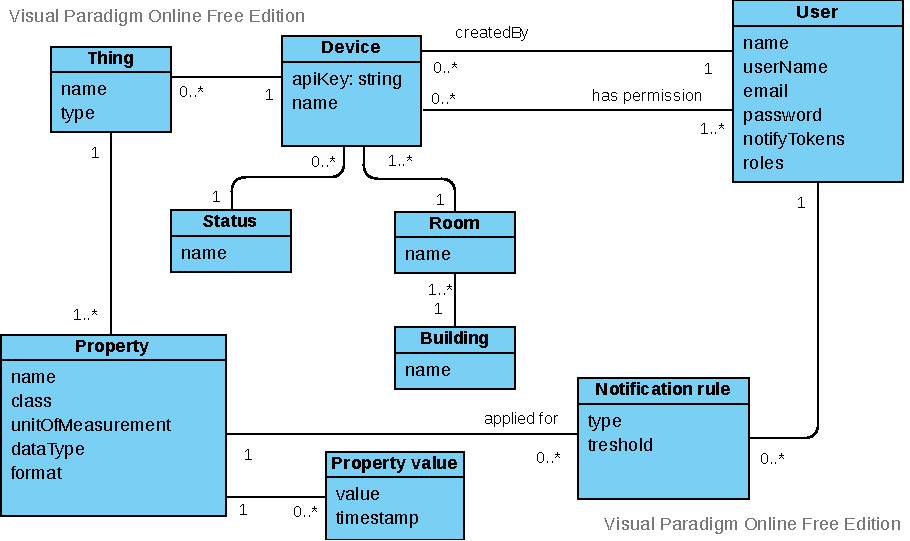
\includegraphics[width=\textwidth]{img/domain.pdf}
    \caption{  \label{domain-model}Doménový model}
\end{figure}
\begin{itemize}
    \item \textbf{Uživatel (User)} - osoba, která interaguje se systémem pomocí uživatelského rozhraní.
    \item \textbf{Zařízení (Device)} - fyzické zařízení, které komunikuje s Platformou a dále se děli na věci.
    \item \textbf{Stav (Status)} - v jakém stavu se zařízení nachází (např. odpojeno).
    \item \textbf{Věc (Thing)} - logické uskupení vlastností, např. meteostanice.
    \item \textbf{Vlastnost (Property)} - určitá veličina, jejíž hodnota se odesílá na Platformu (např. teplota), která případně umožňuje být Platformou změněna/nastavena.
    \item \textbf{Hodnota vlastnosti} - hodnota v určitém časovém okamžiku.
    \item \textbf{Budova (Building)} - místo, které se dále dělí na místnosti.,
    \item \textbf{Místnost (Room)} - uskupení více zařízení.
    \item \textbf{Notifikační pravidlo} - za jaké podmínky se má uživateli odeslat notifikace.
\end{itemize}


\subsection{Případy užití}
Tato kapitola popisuje identifikované případy užití, které současně slouží jako podklad funkčních požadavků kladených na řešení. Figurují v nich následující aktéři:
\begin{itemize}
    \item Neautorizovaný uživatel - představuje nepřihlášeného uživatele webového rozhraní.
    \item Uživatel - přihlášený uživatel webového rozhraní.
    \item Administrátor - autentizovaný uživatele s vyšším stupněm oprávnění.
    \item Zařízení - koncové zařízení komunikující s Platformou
\end{itemize}

\begin{figure}[htbp]
    \centering
    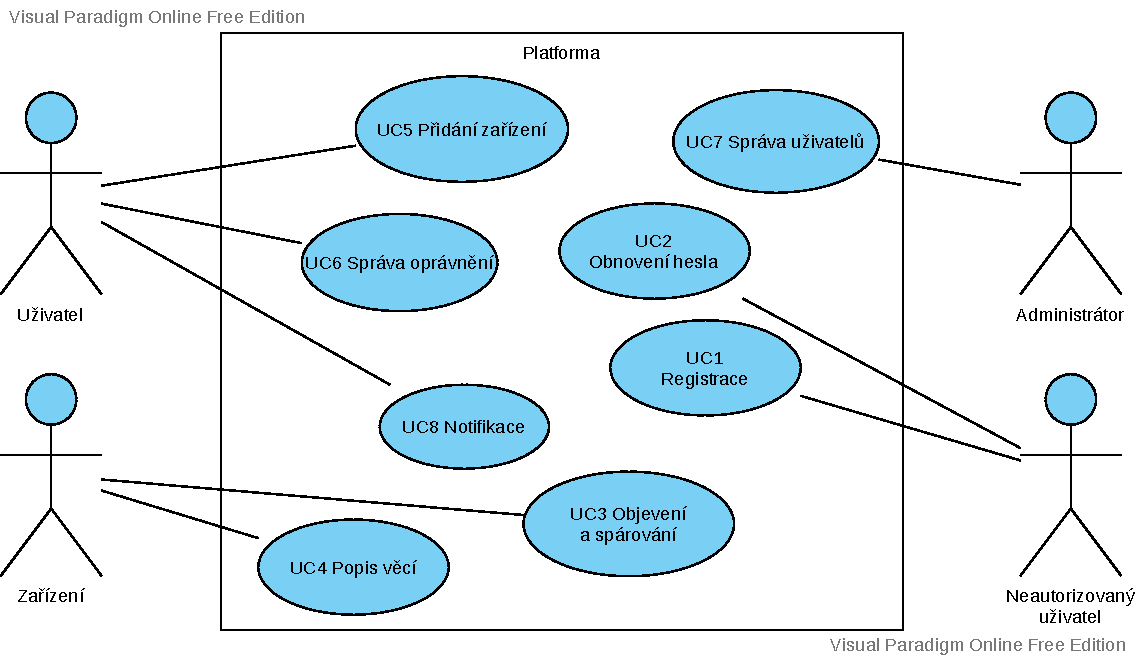
\includegraphics[width=0.9\textwidth]{img/use_case.pdf}
    \caption{Případy užití}
\end{figure}

\paragraph{UC1 Registrace uživatele}
Neautentizovaný uživatel vyplní registrační formulář obsahující jméno, přijmení, uživatelské jméno, heslo a email. Při zpracování požadavku na serveru bude zajištěna unikátnost uživatelského jména a emailu napříč databází. Uživatel bude informován o úspěchu/neúspěchu akce. Po úspěšné registraci bude automaticky přihlášen, pokud nezrušil ve formuláři zaškrtávátko \uv{Automaticky přihlásit}. Následně mu bude odeslán uvítací email na zadanou emailovou adresu.

\paragraph{UC2 Obnovení hesla}
Součástí přihlašovacího formuláře bude odkaz na stránku pro obnovení zapomenutého hesla, kde bude uživatel dotázán na emailovou adresu, kterou použil při registraci. Po zadání, pokud daná emailová adresa je součástí některého uživatelské účtu, bude odeslán email s odkazem pro obnovu hesla. Na tomto odkazu bude uživatel vyzván k zadání hesla nového.

\paragraph{UC3 Objevení a spárování nového zařízení}
Zařízení, pokud ještě není spárované s Platformou, po zapnutí vyzve uživatele k zadání svého uživ. jména k platformě. Toto zadání bude umožněno vytvořením Wifi přístupového bodu, na kterém poběží kaptivní portál - po připojení telefonem/počítačem se automaticky zobrazí webová stránka s formulářem pro zadání údajů. Následně se zařízení připojí k Platformě, ohlásí jaké má věci, popíše jejich vlastnosti, a bude ji informovat, kterému uživateli (podle zadaného uživ. jména) má zobrazit možnost přidání nového zařízení. Pokud si uživatel dané zařízení přidá (viz. \hyperref[UC5]{UC5}), Platforma následně odešle zařízení API klíč, které si ho uloží a přihlásí se pomocí toho klíče k Platformě (nyní je spárované).

\paragraph{UC4 Popis věcí}
Zařízení při ohlašování definice věcí a jejich vlastností musí oznámit mimo jiné typ věci. Platforma bude podporovat kromně generického (generic) typu další 3 typy věcí, pro které bude speciální zobrazení v uživatelském rozhraní:
\begin{itemize}
    \item \textbf{Switch} - přepínač, který se nachází ve stavu on/off. V rozhraní bude věc reprezentována dvoustavovým přepínačem, který při kliknutí odešle změnu o stavu na druhý, než ve kterém se aktuálně nachází. (využití např. vypínač světla)
    \item \textbf{Activator} - spínač, který má pouze jeden stav. V rozhraní bude věc reprezentována tlačítkem, které na stisk odešle aktivaci zařízení. (využití např. ovladač pojízdné brány)
    \item \textbf{Sensor} - v rozhraní bude reprezentován jako widget zobrazující aktuální hodnotu první vlastnosti. Po rozkliknutí se zobrazí graf vizualizující průběh hodnoty v čase za posledních 24h.
    \item \textbf{Generic} - obecný typ, u kterého zařízení popíše strukturu, datové typy a názvy příslušných vlastností. V uživatelském rozhraní bude věc reprezentována jako Widget, který po kliknutí zobrazí Dialogové okno umožňující zobrazení a ovládání všech vlastností dle konfigurace.
\end{itemize}

\paragraph{UC5 Přidání zařízení}
\label{UC5}
Uživateli na stránce \uv{Správa zařízení}, v případě že bude detekováno nové zařízení, v sekci \textit{Přidat zařízení} se zobrazí (bez nutnosti aktualizace stránky) možnost přidat nové zařízení. Při kliknutí na tlačítko přidat se zobrazí jednoduchý formulář pro zadání umístění a názvu zařízení - bude předvyplněn název, který ohlásilo zařízení. Uživatel formulář potvrdí, systém následně vytvoří dané zařízení, přidá uživateli k němu oprávnění a na stránce \uv{Ovládání} už bude uživatel moci sledovat aktuální stav věcí a případně je i ovládat (pokud to umožňují).

\paragraph{UC6 Oprávnění}
Uživatel na stránce \uv{Správa zařízení} v sekci \textit{Správa} bude mít zobrazena všechna zařízení, ke kterým má uživatel oprávnění. Rozhraní umožní pro každé zařízení, ke kterému má příslušné oprávnění editaci, jeho smazání a pomocí formuláře editaci - názvu, umístění a změnu oprávnění pro jednotlivé uživatele. Tyto oprávnění budou rozděleny na tři úrovně:
\begin{itemize}
    \item Čtení - uživatel může si zobrazit veškeré údaje o zařízení.
    \item Ovládání - uživatel může zařízení ovládat.
    \item Správa - uživatel může editovat veškeré informace o zařízení (včetně oprávnění).
\end{itemize}

\paragraph{UC7 Správa uživatelů}
Administrátor má k dispozici stránku \uv{Správa uživatelů}, kde se mu zobrazí seznam všech registrovaných uživatelů. Jednotlivé uživatele může smazat a pomocí formuláře editovat všechny jejich osobní údaje a změnit heslo pro přihlášení.

\paragraph{UC8 Notifikace}
Rozhraní umožní uživateli nastavit pravidlo pro libovolnou věc, při kterém se odešle Web Push notifikaci (technologie umožňující serveru odeslat upozornění do prohlížeče klienta \cite{web-push}) na jeho zařízení. Pro nastavení bude zobrazený formulář umožňující výběr z vlastností dané věci, po vybrání se zobrazí výběr akce, při jejímž splnění chce uživatel obdržet notifikaci (překročení hodnoty / vždy / hodnota bude rovna) a případné pole pro zadání limitní hodnoty. Dále půjde zobrazit rozšířené nastavení pro konkrétní notifikační pravidlo umožňující nastavení času a konkrétních dnů v týdnu, kdy bude pravidlo platné (ve výchozím stavu bude vždy). Těchto pravidel si bude moci nastavit libovolný počet pro každé zařízení, ke kterému má oprávnění pro čtení.



\subsection{Nefunkční požadavky}

\paragraph{N1 Řešení spustinelné na Linux systému}
Systém bude možno provozovat na Linuxovém serveru (Debian) a také na platformě Raspberry Pi (verze 3B+/4, OS Raspbian).

\paragraph{N2 Responzivní webové rozhraní}
Aplikace bude nabízet responzivní webové rozhraní přizpůsobené pro zobrazení na mobilních zařízeních i stolních počítačích. Uživatelské rozhraní bude kompatibilní s prohlížeči Mozilla Firefox verze 80, Chrome verze 80 a Safari na iOS. Dále bude implementovat tzv. PWA (Progresivní webová aplikace) - bude využívat cache pro statické soubory pro rychlé načítání, spustitelné offline a na zařízení Android půjde v aplikaci chrome přidat na plochu a následně vypadat jako nativní aplikace.

\paragraph{N3 Rozhraní realizováno jako SPA}
Single page application (SPA) je webová aplikace, která utilizuje JavaScript tak, aby při interakci v rámci aplikace se nemusela načítat celá stránka, ale pouze chytře překresluje potřebné části. Výsledkem je mnohem přijemnější uživatelský zážitek, než při čekání na stažení a překreslení celé stránku po kliknutí na odkaz.

\paragraph{N4 Validace}
Uživatel v průběhu vyplňování formulářů v rozhraní obdrží interaktivní zpětnou vazbu v případě zadání nevalidních údajů. Interaktivní zpětnou vazbou jsou myšleny následující scénáře při průchodu formuláře:
\begin{itemize}
    \item Zadání nové hodnoty a opuštění pole - bude provedena validace a v případě nevalidního vstupu, bude uživatel vizuálně  upozorněn.
    \item Editace již zadané hodnoty v poli - validace bude provedena po každé změně (stisknutí klávesy), uživatel bude vizuálně upozorněn v případě nevalidního vstupu.
\end{itemize}

\paragraph{N5 Koncová zařízení}
Bude specifikován protokol, pomocí kterého s platformou budou zařízení komunikovat včetně definování schématu komunikace. Platforma umožní připojení libovolného zařízení, pokud použije definovaný protokol a bude se řídit schématem pro komunikaci.

\paragraph{N6 Výkonnostní požadavky}
Systém bude stabilní a zvládne obsluhovat stovku zařízení, kde každé bude odesílat změnu stavu s periodicitou 30 vteřin. Při tomto dlouhodobém zatížení nebude docházet k pádům systému ani k výraznému zpoždění komunikace (RESTful požadavky pod 500 ms).

\paragraph{N7 Konfigurace systému}
Veškerá konfigurace týkající se externích služeb jako jméno a heslo do databáze, číslo portu pro komunikaci atd. bude konfigurovatelné pomocí promněných prostředí (env variables). Detailní popis promněných bude obsažen v instalační příručce.


\subsection{Vybrané technologie}
Tato sekce se věnuje výběru protokolu pro komunikaci se zařízeními a programovacího jazyka, ve kterém bude řešení implementováno včetně výběru příslušných knihoven.

\subsubsection{Komunikační protokol}
Komunikačních protokolů je velké množství a jeho výběr přímo závisí na použitém přenosovém médiu. Při použití specializovaných sítí jako LoRa nebo Zigbee, nemáme moc velkou flexibilitu ve výběru. Zařízení podporující tyto specializované sítě jsou poměrně drahá, ale umožňují běh na baterii. Zatímco využití Wifi sítě nám dává obrovskou flexibilitu ve výběru protokolů a zařízení podporující připojení k Wifi nebyly nikdo více cenově dostupné jako dnes. Primárně z finančních nároků a možnosti využití stávající Wifi infrastruktury v domácnosti jsem se rozhodl pro Wifi jako bezdrátové médium. Současně díky přímé podpoře IP protokolu nebudu muset vytvářet bridge mezi serverem a sítí se zařízeními jako např. při použití Bluetooth či LoRa.

Z protokolů pro komunikaci je dnes nejpoužívanější HTTP, který ale nativně nepodporuje obousměrnou komunikaci, kdy zařízení může poslat zprávu serveru a stejně tak server zprávu zařízení, kterou pro ovládání zařízení budu potřebovat. Z obousměrných protokolů se velmi osvědčil WebSocket, který lze velmi snadno kombinovat s HTTP. Jedná se o protokol postavený nad TCP, který naváže spojení a obě strany mohou posílat zprávy \cite{websocket}. Je to velmi pěkné řešení pro posílání zpráv, ale neumožňuje nativně systematickou filtraci nebo odběr pouze určitých zpráv a nepočítá s během na nespolhlivých zařízeních. Proto přímo pro IoT vznikl otevřený síťový protokol MQTT, kterým jsem si zvolil jako komunikační protokol, jehož specifikaci vydává nezisková organizace \textit{OASIS}. Využívá asynchroní vzor \textit{publish-subsribe} (v podstatě rozděluje akci na dvě událost - vytvoření akce a její obsluhu) a byl speciálně navržen pro potřeby běhu na jednoduchých embeded zařízení s minimálním datovým tokem. Podrobný přehled všech protokolů využívaný pro IoT viz. \cite{protocols}.

\begin{figure}[htbp]
    \centering
    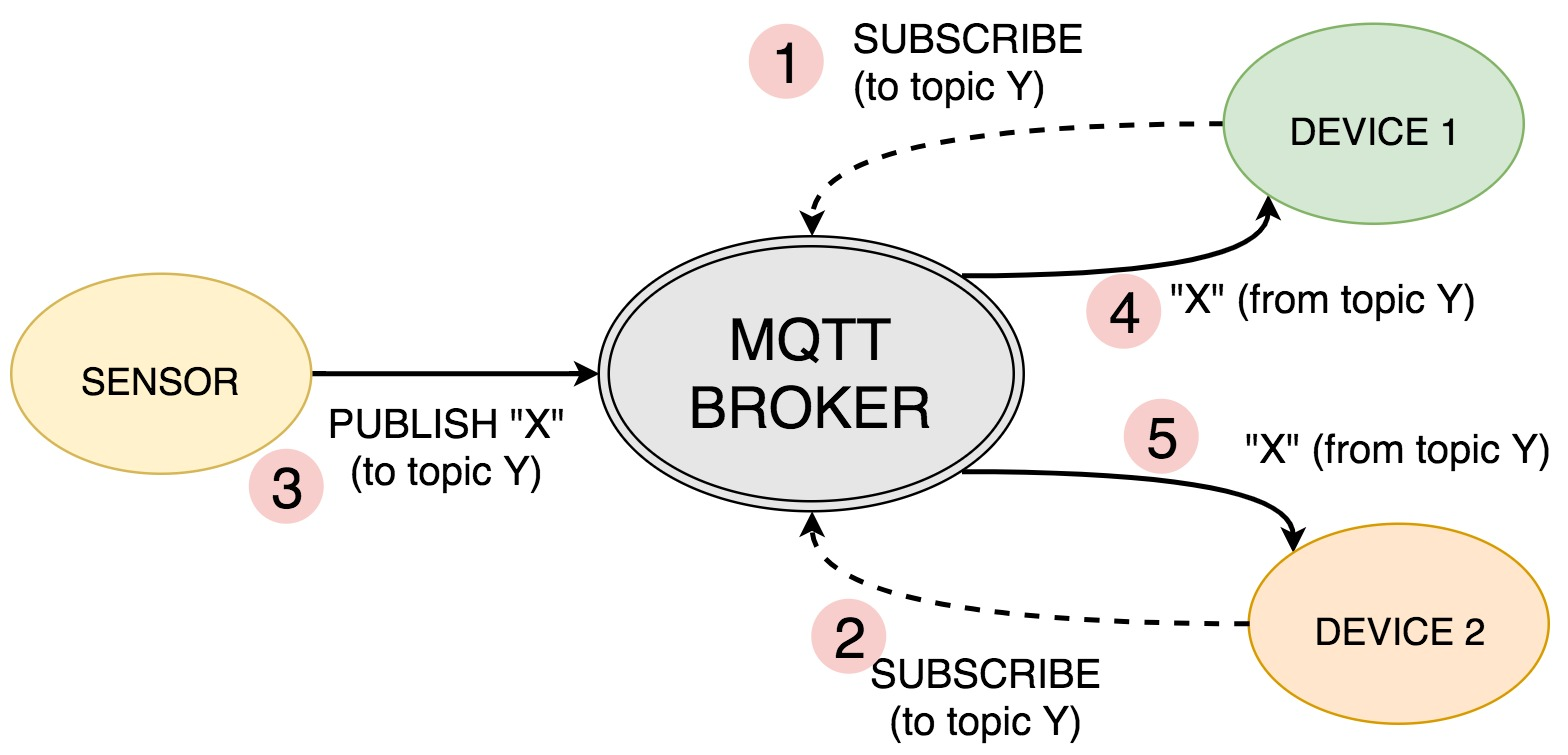
\includegraphics[width=0.7\textwidth]{img/mqtt-communication.jpeg}
    \caption{Ukázka komunikace MQTT \cite{img-mqtt-communication}}
\end{figure}

\label{mqtt-description}
MQTT se vyvýjí již od roku 1999 a momentálně nejpoužívanější verzí je 3.1.1, pro kterou vznikla specifikace v roce 2014. Protokol primárně běží nad TCP/IP, ale lze využít v jakékoliv síti, kde je zaručeno správné pořadí dat, beztrátovost a obousměrnost komunikace. Protokol definuje 2 typy entit: \uv{MQTT broker} a \uv{klient}. MQTT broker je server, který přijímá všechny zprávy od připojených klientů a přeposílá je příjemncům (klientům). MQTT klient je jakékoliv zařízení (od embeded až po server), které komunikuje s brokerem přes síť. \cite{mqtt}

Posílaná data jsou hierarchicky rozdělena do tzv. témat. Téma je textový řetězec o maximální délce 65\,536\,Bytů s oddělovačem lomítko (ukázka \uv{house/bedroom/light}). Pokud klient chce odeslat (publish) data, tak pošle zprávu brokeru s daty a tématem, do kterého zpráva patří. Broker potom zprávu odešle všem klientům, kteří jsou přihlášení k odběru (subscribe) z daného tématu. O odběr se klient musí přihlásit a to buď přímo specifikuje plný název topicu nebo částečný s použitím zástupných znaků. MQTT počítá s případnou nespolehlivostí koncových zařízení či sítě, a proto umožňuje klientovi při přihlášení definovat \uv{Last Will and Testament} (\hypertarget{LWT}{LWT}). Při přihlášení klient oznámí téma a zprávu, která se odešle v případě nesprávně odpojeného klienta (výpadek sítě / chyba zařízení). Takto lze notifikovat ostatní zařízení, že došlo ke ztráně spojení s daným klientem. \cite{mqtt}

Broker podporuje 3 třídy QoS (Quality of service), kterou lze specifikovat pro každou zprávu jednotlivě v závisloti na její důležitosti. Seřazeny jsou vzestupně dle náročnosti na systém (overhead) \cite{mqtt}:
\begin{itemize}
    \item \textbf{0 - Maximálně jednou} - zpráva je odeslána pouze jednou a klient ani broker nijak nepotvrzují její přjetí
    \item \textbf{1 - Alespoň jednou} - zpráva je odeslaná několikanásobně, dokud není potvrzené její přijetí
    \item \textbf{2 - Právě jednou} - odesílatel a příjemce navazují dvoucestný hand-shake, aby bylo zaručeno přijmutí zprávy právě jednou
\end{itemize}


\subsubsection{Programovací jazyk}
Programovacích jazyků je dnes na trhu dostupných stovky a každý má své specifické pozitivní i negativní vlastnosti. Při výběru je tedy vždy potřeba zohlednit jeho přínost pro použití na daném projektu. Kromě jazyka samotného je příhodné analyzovat dostupné knihovny a frameworky, které lze v projektu použít a značně tak urychlit celkový vývoj. Pro implementaci této práci byl zvolen jazyk JavaScript konkrétně jeho nadmnožina TypeScript a to z několika důvodů.

Vzhledem k povaze zvoleného protokolu pro komunikaci se zařízeními, jenž je založený na asynchronních zprávách, je JavaScript velmi vhodný, protože je založený na asynchronní event-driven \cite{nodejs} architektuře. Tato architektura nabízí velice elegantní přístup pro zpracování akcí, kde se musí čekat na výsledek jako např. u síťové komunikace či právě asynchronních zpráv. V tradičním jazyce jako Java nebo C++ se toto čekání musí řešit pracným vytvořením nového vlákna, které čeká na výsledek a následným zpracováním. V NodeJS je programátor od této problematiky odstíněn a může se tak plně věnovat tvorbě aplikační logiky, aniž by měl znalosti a zkušenosti s vícevláknovým programováním.

JavaScript je jediný programovací jazyk, který umožňuje psaní jak serverových aplikací, tak i uživatelského rozhraní formou webové stránky a jeho přímé vykonávání ve webovém prohlížeči klienta. Využití jednotného jazyka pro vývoj serveru i uživ. rozhraní přináší obrovskou výhodu v podobě možnosti sdílet nejenom definice pro objekty, ale i přímo části kódu. Toto je velmi vhodné například pro jednotné validace formulářů, různé datové transformace a sdílení aplikační logiky pro frontend \uv{optimistické aktualizace} (aktuální trend, nečekat na potvrzení požadavku ze serveru, ale rozhraní aktualizovat, jako by požadavek byl úspěšný a pouze v případě neúspěchu zobrazit stav ze serveru). Dále jednotný jazyk umožňuje programátorům při vývoji v případě potřeby pohodlně pracovat na obou částech aplikace, aniž by se museli učit nový jazyk.

\paragraph{TypeScript} Je nadmnožina JavaScriptu, která navíc přidává komplexní typový systém \cite{ts} a rozhodl jsem se ho využít jako hlavní programovací jazyk jak pro backend tak i frontend. Jedná se o OpenSource jazyk vyvíjený společností Microsoft, který jeho vznikem chtěl usnadnit přechod C\# a .NET vývojářům k webovým aplikacím \cite{ts}. Mnoho lidí z JavaScript komunity považuje TypeScript jako kontroverzní počin, protože přidává složitost k velmi elegantnímu jazyku a zvyšuje časovou náročnost vývoje. Já jsem dlouhou dobu tento názor také zastával, ale v posledních letech při práci na větších projektech a díky zkušeností z jiných jazyků (včetně striktně typových jako C++ a Java), jsem změnil svůj názor ve prospěch TypeScriptu. Souhlasím, že na první pohled prodlužuje dobu vývoje. Programátor musí psát věci navíc oproti čistému JavaScriptu, ale v dlouhodobém životním cyklu projektů se tato práce \uv{na víc} mnohonásobně vrátí. A to v podobě statické kontroly typů, která minimalizuje riziko pádu aplikace a umožňuje  lepší statickou analýzu kódu, a dále jako největší přínos pro mne jako programátora TypeScript přináší funkční \uv{našeptávání} ve vývojovém prostředí, které pro JavaScriptu i přes veškeré snahy bohužel funguje ve velmi omezené míře.

\subsubsection{Server}    %https://nodejs.org/en/docs/
%spousta jazyků, pro koncepsi asynchroních messages MQTT a Websocket se hodí NodeJS
Pro běh JavaScript na straně serveru existuje několik prostředí např. SpiderMonkey, NodeJS či Rhino. Pro realizaci bylo zvoleno prostředí NodeJS, které má pravděpodobně aktuálně největší a nejaktivější komunitu ze všech servrových prostředí pro běh aplikací napříč programovacími jazyky. Pro správu knihoven používá balíčkovací systém npm (jsou i jiné alternativy), ze kterého se stal největší ekosystém na světě, který je zastřešený neziskovou společností \uv{npm, Inc.} provozující centrální repozitář se všemi dostupnými moduly pro NodeJS. Díky sve centralizaci je velmi jednoduchý na používání, ale v posledních letech, kdy se JavaScript zpopularizoval a nyní je jedním z nejoblíbenějších jazyků \cite{survey-languages}, ukázala se centralizace jako poměrně nešťastné řešení kvůli vysokým nákladům na provoz infrastruktury. Pro představu velikosti ekosystému: npm v roce 2020 obsahoval 1\~200\~000 modulů a druhý největší systém RubyGems \uv{pouhých} 350\~000 \cite{modulecounts}. Všechny moduly jsou k dispozici zcela zdarma a díky takto aktivní komunitě lidí, kteří dávají k dispozici své knihovny ostatním, je vysoce pravděpodobné, že pokud chceme řešit nějaký problém, tak na něj již existuje knihovna.

%https://expressjs.com/
\paragraph{ExpressJS}\label{expressjs} Platforma bude implementovat RESTful webové rozhraní a pro jeho implementaci byl zvolen minimalistický framework ExpressJS. První jeho verze vznikla již v roce 2010 a do dnes je mezi vývojáři velmi oblíbený a v mnohém ovlivnil směr vývoje většiny frameworků. Jeho největší výhoda je vysoká flexibilita. Nabízí pouze základní definici způsobu pracování s HTTP požadavky a možnost registrovat tzv. middleware - software, který rozšiřuje funkcionalitu. Veškerá funkcionalita je dodávána pomocí middlewarů, které jsou k dispozici jako moduly. Vývojář si tedy může výsledný server poskládat přesně dle svých představ, kterých existují desítky vytvořených přímo od autorů a další stovky od komunity. \cite{expressjs}


\paragraph{AgendaJS} Knihovna pro perzistentní plánování úkolů pro NodeJS \cite{agendajs}. Umožňuje zpracování/plánování/perzistenci úkolů a jejich opětovné spouštění v případě chyby \cite{agendajs}. Tato knihovna bude primárně využita pro zajištění odeslání emailů a pro spouštění případných plánovaných akcí. Proč v souvislosti s odesláním emailů? Jejich zpracování je závislé na třetí straně - emailovém serveru, který nemusí být vždy dostupný. Pokud systém bude mět odeslat email, tak tímto způsobem bude zajištěno, že i v případě selhání bude email opětovně odeslán, jakmile to bude možné.

\paragraph{Socket.IO}\label{socketio} Pro zajištění aktualizace rozhraní v reálném čase bude využita knihovna SocketIO umožnující navázání obousměrného. Vyznačuje se vysokou spolehlivostí a rychlostí umožňující real-time komunikaci. Jedná se o velice populární a časem ověřené řešení, které zajišťuje kompatibilitu i s prohlížeči nepodporující moderní technologii WebSocket.


\subsubsection{Uživatelské rozhraní}
% React + Redux
Prvním bezesporu světoznámým průkopníkem ve světě JavaScriptu pro tvorbu uživatelského rozhraní byla knihovna \textit{jQuery}, která existuje dodnes, ale spíše se již považuje za přežitek doby. Dnes existuje obrovské množství Frameworků a knihoven pro tvorbu frontendu, ať pro tvorbu na straně serveru nebo přímo na straně uživatele v prohlížeči. Trend dnešní doby je přesouvat generování rozhraní na stranu uživatele, jak kvůli snížení výkonnostních nároků na server, tak spíše kvůli lepší odezvě a uživatelskému zážitku. Mezi nejznámější JavaScriptové frameworky patří bezpochyby Angular, Vue.js, Svelte a nesmím zapomenout na React, který je sice knihovna, ale řadí se na stejnou úroveň. Já jsem si zvolil jako hlavní prostředek pro tvorbu rozhraní React, právě proto že se jedná o knihovnu. Framework se vyznačuje tím, že vynucuje určité problémy řešit jistým způsobem bez možnosti volby. Má to své výhody a nevýhody a do větších týmů bych rozhodně volil raději framework. Tento projekt ale budu vytvářet primárně sám a mám velice rád flexibilitu a možnost volby. V začátcích to bývá časově náročnější, ale vidím v tom obrovskou možnost osobního růstu, protože při každé volbě musím hodnotit výhody/nevýhody a nakonec retrospektivně vidím následky svých rozhodnutí. Mimo to za vývojem Reactu stojí Facebook a je používán největšími technologickými spočnostmi světa (Yahoo!, Nextflix a Airbnb \cite{react-companies}), takže je jistá jeho dlouhodobá podpora a od roku 2013, kdy byla vydána první verze, je dobře odladěný a ověřený.

\paragraph{React} Je deklarativní, efektivní a flexibilní knihovna pro tvorbu rozhraní. Kód dělí do malých izolovaných částí kódu nazvaných \uv{komponenty}, které se skládají do sebe a mohou tvořit komplexní uživatelská rozhraní. Pro vysoký výkon využívá techniku virtuálního DOM - nejprve si vytvoří virtuální strom podoby rozhraní v paměti, který následně porovná s aktuální podobou vykreslenou v prohlížeči a zmanipuluje pouze ty části, které se od posledního vykreslení změnily. Díky tomu je velice efektivní a dokáže vykreslovat komplexní stránky s obrovským množstvím dat. \cite{react}